\documentclass{article}

\usepackage[americanvoltages,siunitx]{circuitikz}

\usepackage{menukeys}

\usepackage{hyperref}



\usepackage{color,soul}
\definecolor{lightblue}{rgb}{.90,.95,1}
\sethlcolor{lightblue}

\usepackage{graphicx}
\graphicspath{ {./images/} }

\usepackage{fancyhdr}
\chead{Written by Neil Johari}

\usepackage{ifthen}

\makeatletter
  \def\pgf@circ@drawvoltagegenerator{
    \ifpgf@circuit@bipole@voltage@below
        coordinate (pgfcirc@Vcont1) at ($(\ctikzvalof{bipole/name}.center) ! \ctikzvalof{voltage/bump a} ! (\ctikzvalof{bipole/name}.-120)$)
        coordinate (pgfcirc@Vcont2) at ($(\ctikzvalof{bipole/name}.center) ! \ctikzvalof{voltage/bump a} ! (\ctikzvalof{bipole/name}.-60)$)
    \else
        coordinate (pgfcirc@Vcont1) at ($ (\ctikzvalof{bipole/name}.center) ! \ctikzvalof{voltage/bump a} ! (\ctikzvalof{bipole/name}.120)$)
        coordinate (pgfcirc@Vcont2) at ($ (\ctikzvalof{bipole/name}.center) ! \ctikzvalof{voltage/bump a} ! (\ctikzvalof{bipole/name}.60)$)
    \fi

    \ifpgf@circuit@europeanvoltage
        \ifpgf@circuit@bipole@voltage@backward
            (pgfcirc@Vcont2)  -- node[currarrow, sloped,  allow upside down, pos=1] {} (pgfcirc@Vcont1)
        \else
            (pgfcirc@Vcont1)  -- node[currarrow, sloped,  allow upside down, pos=1] {} (pgfcirc@Vcont2)
        \fi

    \else % american voltage

        \pgfextra{
            \edef\pgf@temp{\pgfkeysvalueof{/tikz/circuitikz/bipole/kind}}
            \def\pgf@circ@temp{battery}
            \ifx\pgf@temp\pgf@circ@temp
                \def\pgf@circ@batteria{battery}
            \else
                \edef\pgf@circ@temp{battery1}
                \ifx\pgf@temp\pgf@circ@temp
                    \edef\pgf@circ@batteria{battery}
                \else
                    \edef\pgf@circ@batteria{false}
                \fi
            \fi
            \def\pgf@circ@temp{battery1}
        }

        \ifx\pgf@temp\pgf@circ@temp % if it is a battery, must put + and -
            \ifpgf@circuit@bipole@voltage@backward
                (pgfcirc@Vcont2)  node[xshift=2pt,yshift=-6pt] {$-$}  (pgfcirc@Vcont1) node[xshift=-2pt,yshift=-6pt] {$+$}
            \else
                (pgfcirc@Vcont1)  node[xshift=-2pt,yshift=-6pt] {$-$}  (pgfcirc@Vcont2) node[xshift=2pt,yshift=-6pt] {$+$}
            \fi
        \fi

    \fi
}
\makeatother

\title{Extra Lab: LTSpice Lab 1}
\date{Winter 2020}
\author{Engineering 100-950}

\begin{document}

\maketitle

\thispagestyle{fancy}

\section*{Learning Objectives}

\begin{itemize}
  \item You will be able to analyze a basic circuit (one without energy storage elements or dependent sources) by hand using Kirchoff's Laws and Nodal Analysis
\end{itemize}

\section*{Learning Assessments}

\begin{itemize}

  \item What is Ohm's Law?
  \item What are Kirchoff's Voltage Law and Kirchoff's Current Law?
  \item Do Kirchoff's laws apply to non-ohmic devices?
  \item Give a brief description of what nodal analysis is
  \item What are the main steps to performing nodal analysis?
\end{itemize}

\section*{Lab Assignment}

Estimated completion time: ~0.5 hours +- 30 minutes. Please contact an IA if you are having difficulties and are spending more time than this!

I care more about you trying the problems than the fact that your answers are correct. This is a lot of work and you're not expected to do everything correctly!!

\begin{itemize}
  \item You will solve a basic problem set of circuit analysis by hand. These problems are designed to be simple and do not have any "tricks" (30-45 minutes).
\end{itemize}

\section{Introduction}
In lab, you have explored some basic concepts like voltage and current. Additionally, you have built a voltage divider and explored some interesting circuits.

The goal of this lab is to allow you to explore these concepts further to expose you to some of the basics of Electrical Engineering.

This lab is split into two parts. Here you will build the foundation required to understand what's going on under the hood in LTSpice. In lab 2, you will get to actually play with LTSpice.

Many of the concepts we cover here are a preview of what you might learn in a course like EECS 215. If you enjoy this lab and the concepts of it, please consider taking the course!

If you find these concepts easy, consider completing the advanced version of this lab written by Sarah. In that lab, you get to explore basic first order circuits.

\subsection{Credits}
All tables and examples are from the EECS 215 course and book. Much of the wording is almost verbatim from the book, though topics were hand picked and distilled to prepare you for this lab. In particular, the course uses `Circuit Analysis and Design' by Fawwaz T Ulaby, Michael M. Maharbiz, and Cynthia M. Furse.

The assignments are taken directly from Lab 1 of the course, which means that if you choose to take the course, you're already (very slightly) ahead! After this lab you'll have played with LTSpice, which most students entering the course haven't... this will make all the labs significantly easier to work with.

This book can be freely downloaded here. It is not required to complete this lab or understand all the material, but may serve as a helpful reference if you need a more detailed primer than we provide here.

\subsection{Disclaimer}
This lab glosses over topics I believe were not relevant to being able to complete the end goal of simulation with SPICE (which you will do in lab 2 if you choose to continue). A partial list of some topics that this manual hand-waves over is below, and hopefully if you enjoyed this lab you will go on to explore these in more depth in future classes:

\begin{itemize}
  \item Dependent voltage and current sources
  \item Source transforms
  \item Wye-Delta transforms
  \item Resistance and conductance at a material level
  \item Power
  \item Mesh analysis
  \item Supernodes
\end{itemize}

\subsection{Pre-requisites}
I assume you are familiar with the concepts of charge, current, and voltage. If
you are not, please read the `Circuits Primer' on Canvas under \menu{Files >
Labs > Introductory Documents > Circuits\_Primer.pdf}. 

This is an excellent way to intuitively grasp voltage and how it relates to current.


\section{Circuit Basics}
\subsection{Terminology}
Here are some reference tables that will be useful in understanding circuit
diagrams. Figure \ref{fig:si_units} (Table 1-1 from UMF) covers units you might
encounter and their symbols, Figure \ref{fig:si_units2} (Table 1-2 from UMF)
covers SI units, and Figure \ref{fig:circuit_elements} (Table 1-3, UMF) shows common circuit elements.

\begin{figure}[!htbp]
\centering
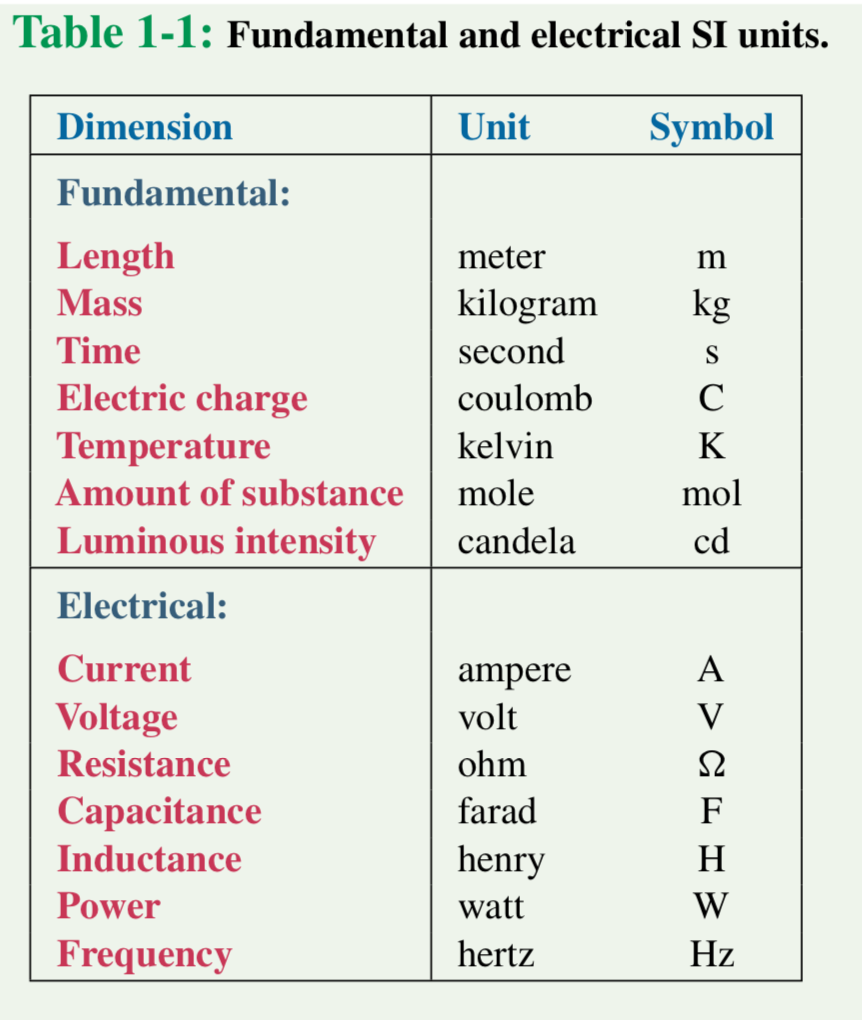
\includegraphics[width=0.5\textwidth]{table_1-1}
\caption{SI Units and Symbols}
\label{fig:si_units}
\end{figure}

\begin{figure}[!htbp]
\centering
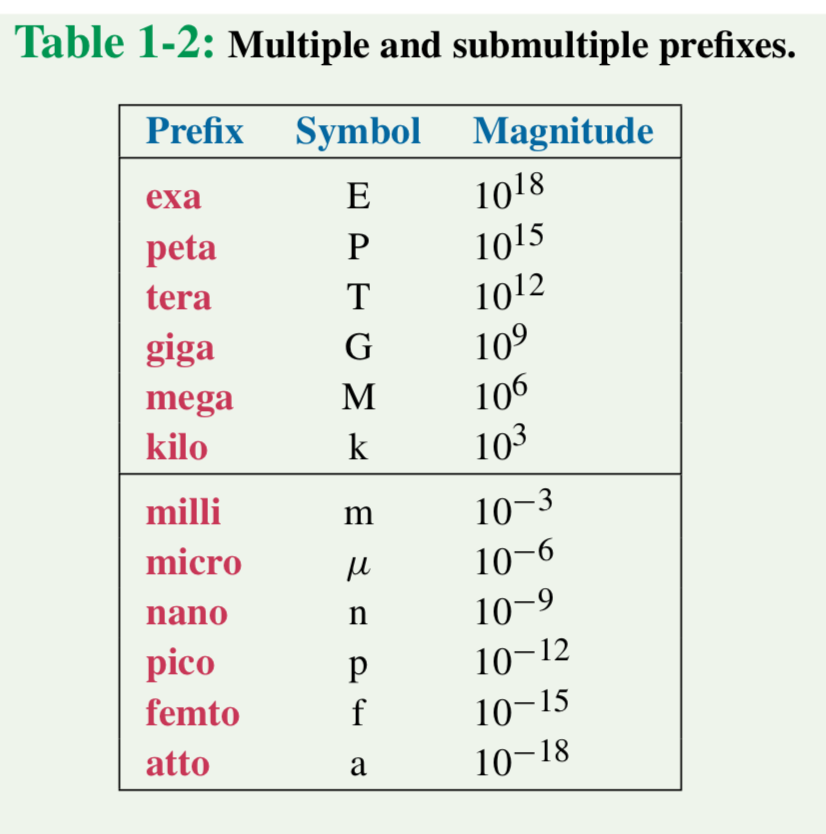
\includegraphics[width=0.5\textwidth]{table_1-2}
\caption{SI Prefixes}
\label{fig:si_units2}
\end{figure}

\begin{figure}[!htbp]
\centering
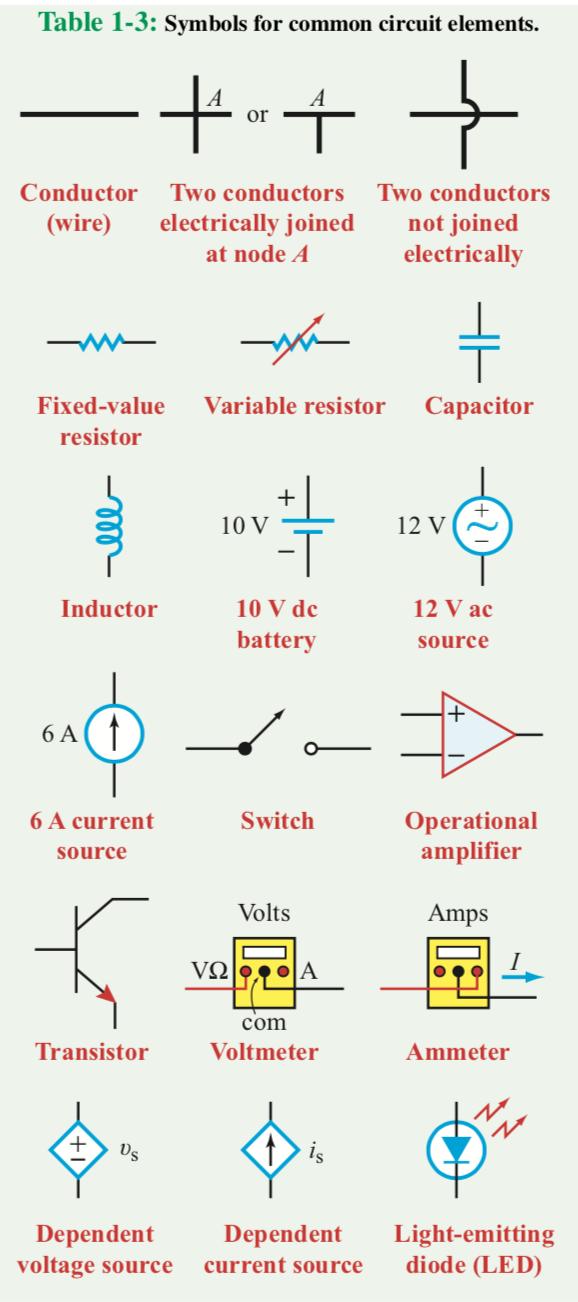
\includegraphics[width=0.5\textwidth]{table_1-3}
\caption{Common Circuit Elements}
\label{fig:circuit_elements}
\end{figure}

Some important terms we will formalize:

\begin{itemize}
  \item Node: An electrical connection point that connects multiple circuit elements
    \begin{itemize}
      \item Note that we often draw things in a way that's easy to visualize, but really anything connected by the same wire with no circuit elements in between is part of the same node.
    \end{itemize}
  \item Branch: Trace between two consecutive nodes with only one element in between them
  \item Loop: Closed path with the same start and end node
  \item Mesh: A restricted kind of loop: it is a loop that encloses no other loops
  \item In series: elements that share the same current
  \item In parallel: elements that share the same voltage
\end{itemize}

\subsection{Reference nodes}
One thing many of you struggled with during labs was understanding the importance of ground.

The big idea is that voltage is by definition between two points. However, for convenience sometimes we like to assign a particular node to be our ground node, so that we can measure all our voltages relative to this.

Say we have a circuit and we are measuring the voltage between two nodes, a and
b. Then $V_{ab} = V_a - V_b$. Now let's say that we make all future measurements
relative to node b... let us assign node b to be our reference point by calling
it ground. Now we are allowed to simply refer to $V_a$ and it is implied that it is relative to ground (node b).

\subsection{The Resistor}
A resistor is a device which impedes current. It always drops voltage.

A resistor is an excellent example of an almost perfect "Ohmic" device. An ohmic
device is one which follows Ohm's Law, $V = IR$, at least for some particular range of current (called the linear region).

Not all devices follow this relationship! Elements like diodes are nonlinear and we cannot use Ohm's law for these.

\subsection{Passive Sign Convention}
There are two ways to assign polarity to an element with current entering it.

We will choose to assign current entering a device to be defined as entering the
(+) side of v. We will not cover power in this lab, but this effectively means
that any circuit elements dissipating power will have a $P > 0$, and any
elements supplying power will have a $P < 0$.

\begin{figure}[!htbp]
\centering
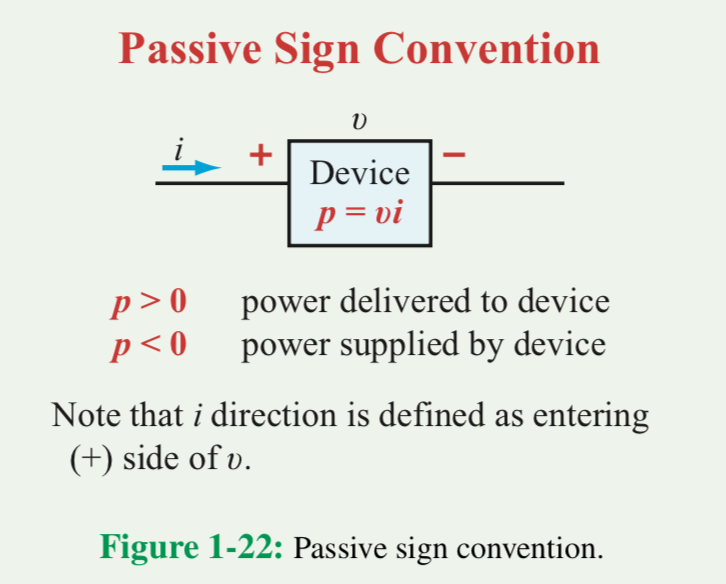
\includegraphics[width=0.5\textwidth]{fig_1-22}
\caption{Passive Sign Convention}
\label{fig:passive_convention}
\end{figure}

\section{Circuit Analysis Fundamentals}
All circuit theory is built on a pretty small set of fundamental laws, of which KCL and KVL are the most important.

The most interesting thing is that these laws are ALWAYS true; they are built upon fundamental laws of conservation of energy. This means that even if you have a non-ohmic device, you absolutely can still write these equations and they will hold.
\subsection{Kirchoff's Current Law (KCL)}
In an ideal circuit, a node is unable to store, generate, or dissipate electric charge. Thus, all current entering a node must equal all current leaving a node.

In other words, the sum of all currents entering a node must equal 0.

\href{https://www.khanacademy.org/science/electrical-engineering/ee-circuit-analysis-topic/ee-dc-circuit-analysis/v/ee-kirchhoffs-current-law}{Here is a good video on KCL}.

\subsection{Kirchoff's Voltage Law (KVL)}

The law of conservation of energy states that if electric charge is moved around a closed loop (where end position = start position), then the net gain or loss of energy must be 0.

Voltage is related to potential energy, thus the algebraic sum of voltages around a closed loop must be 0.

In terms of getting the signs right, follow these two rules and you'll get the right equation every time:

\begin{enumerate}
  \item Go around your loop in a clockwise fashion
  \item Assign a positive sign to your KVL equation if you encounter the (+) side of an element first, and a negative sign if you encounter the (-) side first
\end{enumerate}

If you would like a video on KVL, \href{https://www.khanacademy.org/science/electrical-engineering/ee-circuit-analysis-topic/ee-dc-circuit-analysis/v/ee-kirchhoffs-voltage-law}{here is our recommendation.}

\href{Here is a video showing an example of how we label
voltages}{https://www.khanacademy.org/science/electrical-engineering/ee-circuit-analysis-topic/ee-dc-circuit-analysis/v/ee-labeling-voltages}.

\subsection{Application of Fundamental Laws 1}

Using KVL, KCL and Ohm's Law solve for all unknown currents and voltages in the
circuit in Figure \ref{fig:assignment1}.

\begin{figure}[!htbp]
\centering
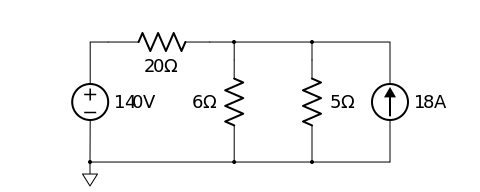
\includegraphics[width=0.5\textwidth]{khan_task}
\caption{Circuit for Application of Fundamental Laws 1}
\label{fig:assignment1}
\end{figure}

\subsection{Bonus Problem: Application of Fundamental Laws 2}

\textit{This problem is not required for completion of this lab because it
  contains two voltage sources. You should still give it a try if you have
time!}

Using KVL, KCL, and Ohm's Law, solve for v1, v2, v3, i1, i2, and i3 in the
circuit in Figure \ref{fig:bonus_assignment}.

\begin{figure}[!htbp]
\centering
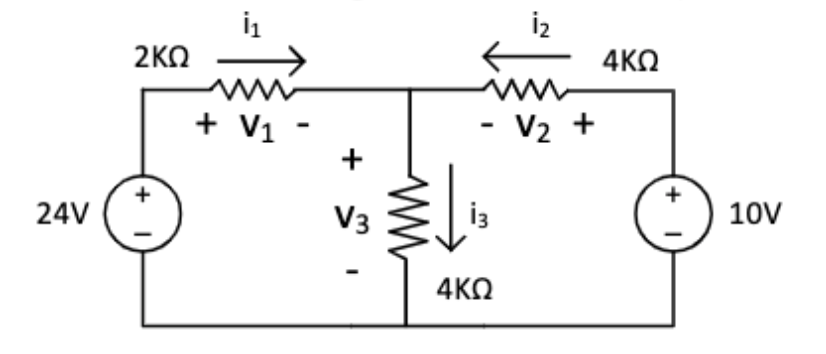
\includegraphics[width=0.5\textwidth]{hw2_1}
\caption{Circuit for Bonus Problem}
\label{fig:bonus_assignment}
\end{figure}


\subsection{Nodal Analysis}

It would be nice to have a codified set of steps to solve for all voltages and currents in a circuit.

If you have taken physics in high school or Physics 240, you know that it can be frustrating to throw KVL/KCL mindlessly at a circuit and hope to get a set of linearly independent equations to solve the circuit problem at hand.

The Node Voltage Method is an organized and efficient way of approaching any circuit and is based off of Kirchoff's Current Law.

The goal of the method we present is a way to mindlessly solve a circuit.

Steps for Nodal Analysis:

\begin{enumerate}
  \item Identify all nodes in the circuit
  \item Choose a ground node
  \item Generate a KCL equation for each non-reference node. An easy way to make this mindless is to always form the sum of currents leaving the node (assigning a negative sign to any current entering the node).
  \item Generate a KVL expression for each voltage source representing the drop between 2 nodes connected by the voltage source
  \item Solve the independent simultaneous equations using a solver program like MATLAB.
\end{enumerate}

Please watch
\href{https://www.khanacademy.org/science/electrical-engineering/ee-circuit-analysis-topic/ee-dc-circuit-analysis/v/ee-node-voltage-method-steps-1-to-4}{this video for a good overview of the process}. The video uses a
slightly different set of steps that perform the same analysis.

\subsection{Example of Nodal Analysis: Battery with Two Parallel Resistors}


\begin{circuitikz} \draw
(0,0) to[battery1, v=\SI{8}{\volt}, i=$i_v$] (0,4)
      to (4,4)
(4,4) to[resistor, l=2<\kilo\ohm>] (4,0)
      to (0,0)
(4,4) to (8,4)
(8,4) to[resistor, l=4<\kilo\ohm>] (8,0)
      to (0,0)
;
\end{circuitikz}

Let us perform the steps listed:
\begin{enumerate}
  \item There are 2 nodes in this circuit (above and below the battery). 
    \begin{itemize}
      \item Note that even though there are 3 branches, all the top wires of the branches connect into a common wire with no circuit elements between them, thus they are part of the same node (the positive terminal of our battery). Similarly, all the bottom
  wires of the branches connect into one wire and form the second node (the
  negative terminal of the battery).
      \item Let's call the bottom node $V_0$ and the top node $V_1$.
    \end{itemize}
  \item Let's just choose the bottom node to be ground (thus the negative terminal of the battery is at 0V).
  \item There is one non reference node. Let's write KCL for it!
    \begin{itemize}
      \item $i_v + \frac{V_1}{\SI{2}{\kilo\ohm}} + \frac{V_1}{\SI{4}{\kilo\ohm}} = 0$
    \end{itemize}
  \item Let's generate a KVL expression for our one voltage source.
    \begin{itemize}
      \item $V_1 - 0 \text{V} = \SI{8}{\volt}$
    \end{itemize}
  \item We can now solve for $V_1$ and $i_v$! Plugging in and solving our system
    yields $V_1 = \SI{8}{\volt}$ (somewhat obviously) and $i_v = \SI{6}{\ampere}$
\end{enumerate}

\subsection{Example of Nodal Analysis: Voltage Divider}

\begin{circuitikz} \draw
(0,0) to[battery1,v=\SI{12}{\volt}] (0,4)
      to[resistor, l_=\SI{1}{\kilo\ohm}] (4,4)
      to (4,2)
      circle[radius=1pt] node[label={right:$V_{out}$}] {}
      to (4,0)
      to[resistor, l=\SI{3}{\kilo\ohm}] (0,0)
;
\end{circuitikz}

You have already explored voltage dividers in lab! To refresh your memory, here
is the formula for a voltage divider with 2 resistors: $V_{out} = \frac{R_2}{R_1 + R_2}$.

Using this formula, we can see from the diagram that we expect $V_{out} =
\frac{3}{4} * 12 \text{V} = \SI{9}{\volt}$. 


Let's use nodal analysis to verify this result! Note that by not labeling
"obvious" nodes (like ones with only a battery separating them from ground), we
can sometimes reduce the number of equations we need to write.

\begin{enumerate}
\item There are 3 nodes in this circuit: on either side of the battery, and $V_{out}$
\item Let's choose the bottom terminal of the battery to be ground. The node at the positive terminal of the battery is clearly 12 Volts then, so we won't bother
labeling it, since it's already solved.
\item There is only one unsolved non-reference node: $V_{out}$. Let's write a KCL
expression for it!
  \begin{itemize}
    \item  $$\frac{V_{out} - \SI{12}{\volt}}{\SI{1}{\kilo\ohm}} + \frac{V_{out} -
  \SI{0}{\volt}}{\SI{3}{\kilo\ohm}} = 0$$
  \end{itemize}
\item Since we didn't bother to label the node above the voltage source and just
directly solved for it, we do not need to write a KVL expression for the
voltage source. 
\item We can now solve for $V_{out}$ to obtain that $V_{out} = \SI{9}{\volt}$, just as expected!
\end{enumerate}

\subsection{Application of Nodal Analysis}

Apply nodal analysis to determine the current I in Figure
\ref{fig:nodal_assignment}. There are
many ways to do this. If you are struggling, watch the video linked before the
assignments! You can use MATLAB to solve the equations if needed, though it
should be trivial to do by hand.

\begin{figure}[!htbp]
\centering
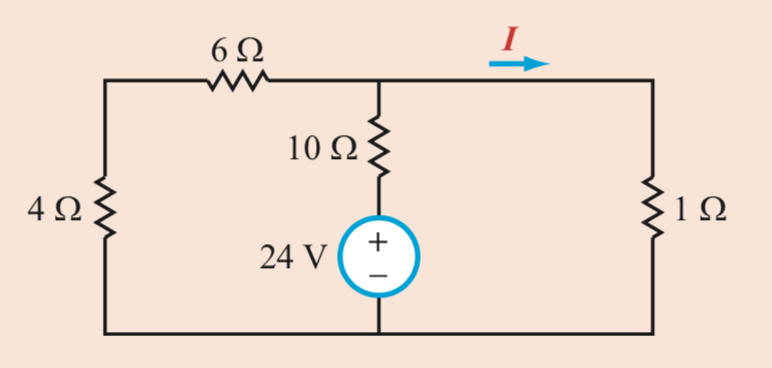
\includegraphics[width=0.5\textwidth]{e_3-1}
\caption{Circuit schematic for assignment on nodal analysis}
\label{fig:nodal_assignment}
\end{figure}

\section*{What to submit for this lab}

\begin{enumerate}

  \item Your solution to "Application of Fundamental Laws 1"
    \begin{itemize}
  \item Include all equations and any diagrams you drew to solve this problem (if any)
    \end{itemize}
  \item  Your solution to "Application of Nodal Analysis"
    \begin{itemize}
      \item Include all equations and any diagrams you drew to solve this problem (if any)
    \end{itemize}
  \item Don't forget to Slack message either Neil or Sarah!
\end{enumerate}

\end{document}
